% Source: https://tex.stackexchange.com/a/250740/6880

\documentclass[varwidth=false, border=2pt]{standalone}

\usepackage{tikz}
\usetikzlibrary{arrows,positioning}

\tikzset{
   % House
   pics/house/.style args={#1/#2/#3}{
   code={
      % Define house parameters
      \newcommand\wallheight{#1}  % 0.65
      \newcommand\roofoverhang{#2}  % 0.15
      \newcommand\roofangle{#3}  % 35

      % Calculate some dependent sizes
      \pgfmathsetmacro\lengthroof{0.5/cos(\roofangle)+\roofoverhang}

      % draw profile of house
      \draw[line width=1pt] (-0.5,\wallheight) -- (-0.5,0) --  (0.5,0) -- (0.5,\wallheight) -- ++(-\roofangle:\roofoverhang) -- ++(180-\roofangle:\lengthroof) -- ++(180+\roofangle:\lengthroof) -- cycle;
    }},
  pics/house/.default=0.65/0.15/35
}

\begin{document}
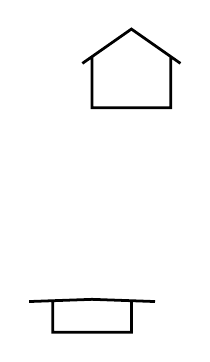
\begin{tikzpicture}

\path (+1.5,-0.85) pic[scale=1.0] {house=0.4/0.3/2};

\draw (2,2) pic[scale=1.0] {house};

\end{tikzpicture}
\end{document}